% !TeX spellcheck = it_IT
\newpage
\section{Progettazione}
La fase di progettazione è tra quella della specifica (cosa fare) e quella della programmazione. Come risultato produce un'\textbf{architettura} che descrive \textbf{come} fare.\\
Possono esserci due livelli di astrazione:
\begin{itemize}
	\item \textbf{Architetturale}: si scompone un sistema in più sottosistemi, ne si identificano e specificano le parti e le interconnessioni
	\item Di \textbf{dettaglio}: indica come la specifica di ogni parte sarà realizzata
\end{itemize}

\begin{definition}[Architettura software]
	L’architettura di un sistema software è la \textbf{struttura} del sistema, costituita dalle parti del sistema, dalle \textbf{relazioni} tra le parti e dalle loro proprietà visibili.
\end{definition}

\begin{definition}[Stile architetturale]
	Uno stile architetturale caratterizza una famiglia di architetture con caratteristiche simili (e.g. client-server, microservizi). Le funzionalità e le interazioni tra i componenti spesso seguono degli standard.
\end{definition}

Un'architettura si sviluppa in diverse \textbf{viste} e \textbf{stili}.

\begin{center}
	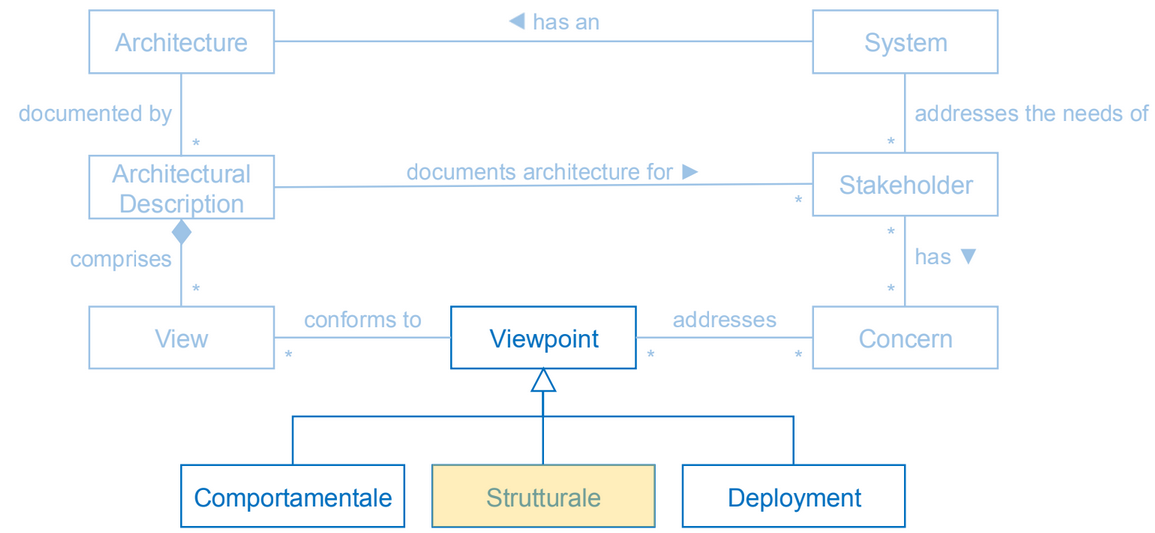
\includegraphics[scale=0.3]{progettazione}
\end{center}

\subsection{Vista comportamentale}
Anche detta \textbf{component-and-connector}, descrive un sistema software come \textbf{composizione di componenti}, compreso di:
\begin{itemize}
	\item \textbf{Interfacce} dei componenti
	\item Caratteristiche dei \textbf{connettori}
	\item Struttura del sistema in esecuzione (flusso dei dati, parallelismo, replicazioni, etc..)
\end{itemize}
Questa vista permette l'analisi delle \textbf{caratteristiche di qualità} a tempo di esecuzione (prestazioni, affidabilità, etc..) e di documentare lo \textbf{stile} dell'architettura.

\subsubsection{Componente}
Una componente software è un'unità concettuale di decomposizione del sistema a tempo di esecuzione. Incapsula un insieme di \textbf{funzionalità} e/o \textbf{dati}, restringendone l'accesso tramite delle \textbf{interfacce}.
\begin{definition}[Componente]
	Una componente software è un'unità di software \textbf{indipendente} e \textbf{riutilizzabile}.
\end{definition}

\begin{definition}[Sistema software]
	Un sistema software è una composizione di componenti software basata sulla connessione di più componenti e realizzata con interfacce dei componenti e connettori,
\end{definition}

\noindent In UML un componente è un \textbf{classificatore} e si compone di:
\paragraph{Porti} I porti ne identificano i punti di interazione. Può essercene più di uno, possono fornire o richiedere una o più \textit{interfacce} e possono avere \textit{nomi} e \textit{molteplicità}.
\begin{center}
	\includegraphics[scale=0.3]{component.png}
\end{center}
I porti possono avere la specifica delle interfacce in due modi:
\begin{itemize}
	\item \textbf{Sintetica}: si indica solo quando è \textit{richiesta} (forchetta) o offerta (\textit{lollipop})
	\begin{center}
		\includegraphics[scale=0.2]{interfaccia_sintetica.png}
	\end{center}
	\item \textbf{Estesa}: si specifica per esteso le operazioni richieste ed offerte
	\begin{center}
		\includegraphics[scale=0.2]{interfaccia_estesa.png}
	\end{center}
\end{itemize}

\paragraph{Connettori}
I connettori sono \textbf{canali di interazione} tra i porti di componenti. Non hanno un descrittore specifico e vengono rappresentati come associazioni. Per dare più informazioni si indica lo \textbf{stile} della connessione o con uno \textbf{stereotipo} o indicando i \textbf{ruoli}.

\begin{center}
	\includegraphics[scale=0.3]{connettori.png}
\end{center}

\subsubsection{Stili}
In questo tipo di vista uno stile architetturale è caratterizzato dalle \textbf{caratteristiche generali} delle componenti e dalle loro \textbf{interazioni} (quindi \textit{porti} e \textit{connettori}).

\paragraph{Pipes \& filters} Questo stile consiste in un flusso di elaborazione di dati che viaggiano lungo le \textbf{pipe} e sono processati dai \textbf{filter}. In particolare i \textit{filter} sono i \textbf{componenti} che trasformano i flussi di dati mentre le \textit{pipe} sono i \textbf{connettori} che fungono da canale di comunicazione unidirezionale bufferizzato che preserva l'ordine di ingresso.
\begin{center}
	\includegraphics[scale=0.3]{pipes_filters.png}
\end{center}

\paragraph{Client-server} Questo stile prevede due componenti che possono essere su macchine diverse. Il \textbf{server} offre il servizio, aspetta le richieste dati ad un porto e può servirne su di esso più alla volta. Il \textbf{client} invia richieste al server e attende una risposta.
\begin{center}
	\includegraphics[scale=0.3]{client-server.png}
\end{center}
Il server in particolare prevede un \textbf{RequestListener} in attesa di richieste e un \textbf{RequestHandler} per ognuna di esse. Quest'ultimo elabora le richieste e:
\begin{itemize}
	\item Se \textbf{stateless} le gestisce ognuna in maniera indipendente
	\item Se \textbf{stateful} consente richieste \textit{composite} che consistono in più richieste \textit{atomiche}, mantenendo un record di esse \textbf{sessione}
\end{itemize}

\paragraph{Master-slave}
Questo stile è una variazione di \textit{client-server} in cui c'è solamente un servente (\textbf{slave}) e un cliente (\textbf{master})

\paragraph{Peer to Peer} Questo stile è una variazione di \textit{client-server} dove tutti i componenti sono sia client che server e avviene uno scambio di servizi alla pari.
\begin{center}
	\includegraphics[scale=0.6]{p2p.png}
\end{center}

\paragraph{Publish-Subscribe} In questo stile i componenti interagiscono in modo \textbf{event-based}. Abbiamo tre tipi di componenti:
\begin{itemize}
	\item \textbf{Publisher}: produce classi di eventi
	\item \textbf{Subscriber}: si iscrive alle classi rilevanti
	\item \textbf{Broker}: smista gli eventi pubblicati
\end{itemize}
Un componente può essere sia \textit{publisher} che \textit{subscriber}. Tra di loro comunicano tramite il \textit{broker}.I publisher non sanno quanti/quali subscriber ci siano e viceversa, garantendo \textbf{scalabilità}.
Questo stile può funzionare in due modi:
\begin{itemize}
	\item \textbf{Push}: il broker invia attivamente i messaggi ai subscriber, controllandone la frequenza
	\item \textbf{Pull}: è il subscriber che manualmente recupera i messaggi dal broker. Migliora la scalabilità e la flessibilità dato che servono meno broker.
\end{itemize}

\begin{figure}[!h]
	\centering
	\begin{minipage}[b]{0.5\textwidth}
		\includegraphics[width=\textwidth]{pub-sub.png}
	\end{minipage}
	\hfill
	\begin{minipage}[b]{0.4\textwidth}
		\includegraphics[width=\textwidth]{pub_sub_full.png}
	\end{minipage}
\end{figure}

\paragraph{Process coordinator}
Un componente funge da \textbf{process coordinator} mentre gli altri sono passivi e non conoscono il loro ruolo nel processo ma si limitano a contribuire. Il \textit{coordinator} conosce la sequenza di passi necessaria, invoca le funzionalità richieste e fornisce una risposta.

\paragraph{Model-View-Controller/Publisher}
Questo stile si basa su tre elementi:
\begin{itemize}
	\item \textbf{Model}: nucleo funzionale che implementa la business logic dell'applicazione e ne rappresenta i dati su cui essa lavora
	\item \textbf{View}: presentazione del model all'utente, possono essercene diverse
	\item \textbf{Controller}: controlla l'input dell'utente e lo traduce in operazioni da eseguire su \textit{model} oppure \textbf{presenter} in alternativa
\end{itemize}
\begin{figure}[!h]
	\centering
	\begin{minipage}[b]{0.4\textwidth}
		\includegraphics[width=\textwidth]{model_view_controller.png}
		\caption*{Controller}
	\end{minipage}
	\hspace{10pt}
	\begin{minipage}[b]{0.4\textwidth}
		\includegraphics[width=\textwidth]{model_view_presenter.png}
		\caption*{Presenter}
	\end{minipage}
\end{figure}

\subsection{Vista strutturale}
Descrive la struttura di un sistema software come insieme di \textbf{unità di realizzazione}, ovvero di codice. Permette di analizzare le \textbf{dipendenze}, progettare i \textbf{test} e valutare la \textbf{portabilità}.\\
La vista strutturale in UML include:
\begin{itemize}
	\item \textbf{Classi} con specifica delle \textit{operazioni} più dettagliata rispetto alla descrizione del dominio
	\item \textbf{Package}
\end{itemize}

\subsubsection{Decomposizione}
\begin{wrapfigure}[7]{r}{5cm}
	\vspace{-1.2cm}
	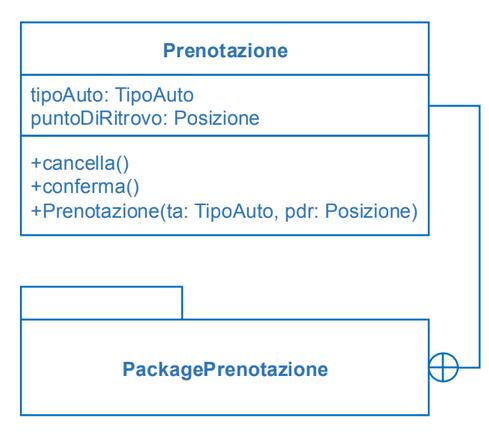
\includegraphics[width=5cm]{decomposizione}
\end{wrapfigure}
Una classe può far parte (essere contenuta in) un package, che a sua volta può far parte di uno più grande. La decomposizione può essere fatta per \textbf{apprendimento} del sistema o per l'\textbf{allocazione del lavoro} e può seguire tre criteri:
\begin{itemize}
	\item Incapsulamento per \textbf{modificabilità}
	\item Supporto alle scelte \textbf{costruisci}/\textbf{compra}
	\item Moduli comuni in \textbf{linee di prodotto}
\end{itemize}

\begin{note}
	La relazione "parte di" si può rappresentare anche con l'inclusione grafica in un package.
\end{note}

\newpage

\subsubsection{Uso}
Un modulo A può usarne un altro B per soddisfare i suoi requisiti. Questo permette di pianificare uno sviluppo incrementale e creare test di unità ed integrazione. Sono permessi i cicli anche se pericolosi.

\begin{center}
	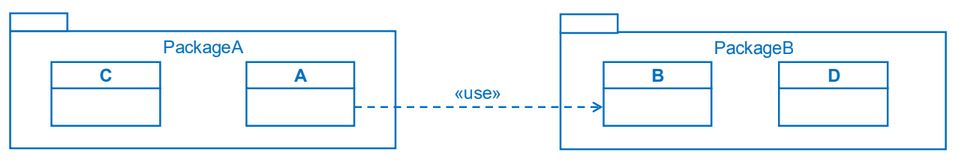
\includegraphics[scale=0.4]{uso}
\end{center}

\subsubsection{Strati}
\begin{wrapfigure}[10]{r}{3cm}
	\vspace{-1cm}
	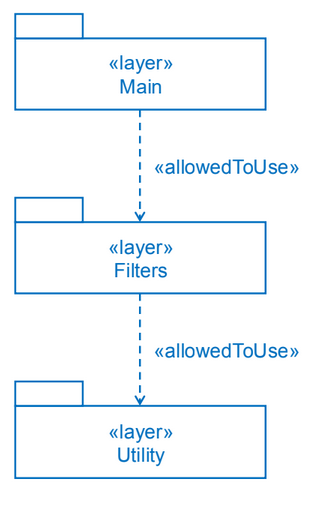
\includegraphics[width=3cm]{strati}
\end{wrapfigure}
Nella vista strutturale a strati ogni elemento (\textbf{strato}) è un insieme coeso di moduli a volte raggruppati in segmenti, il quale offre un'interfaccia pubblica per i suoi servizi. La relazione \textit{allowedToUse} è un caso particolare di quella di uso ed è \textbf{antisimmetrica} e \textbf{non implicitamente transitiva}.\\
Questa vista favorisce modificabilità, portabilità e controllo della complessità.

\subsubsection{Generalizzazione}
In questa vista gli elementi sono i \textbf{moduli} (classi o packages) che hanno una relazione di generalizzazione tra di loro. Permette di rappresentare relazioni di sotto tipo tra classi e la relazione tra un framework\footnote{Collezione di classi, anche astratte, con relazioni d'uso tra loro.} e una sua specializzazione nel caso dei package.

\subsection{Vista di deployment}
Descrive l'allocazione del software su ambienti di esecuzione e permette di valutarne \textbf{prestazioni} e \textbf{affidabilità}. Contiene:
\begin{itemize}
	\item \textbf{Artefatti} prodotti da un processo di sviluppo software o dal funzionamento di un sistema, rappresentati dallo stereotipo \textit{$<<$artifact$>>$}
	\item \textbf{Ambienti di esecuzione} o nodi hardware, rappresentati come \textit{parallelepipedi}
\end{itemize}
Questi elementi possono avere due tipi di relazioni:
\begin{itemize}
	\item \textbf{Dislocazione} di artefatti negli ambienti, rappresentata con il \textit{contenimento}
	\item \textbf{Interconnessione} tra gli ambienti di esecuzione, rappresentate con relazioni stereotipate
\end{itemize}
\begin{center}
	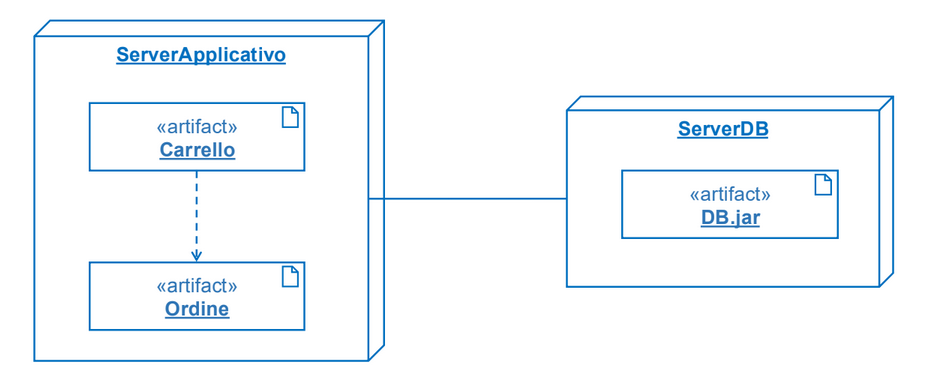
\includegraphics[scale=.4]{deployment}
\end{center}

\subsection{Vista ibrida}
La vista ibrida si compone di quella comportamentale e di quella di deployment su di un'applicazione 3-tier.
\begin{center}
	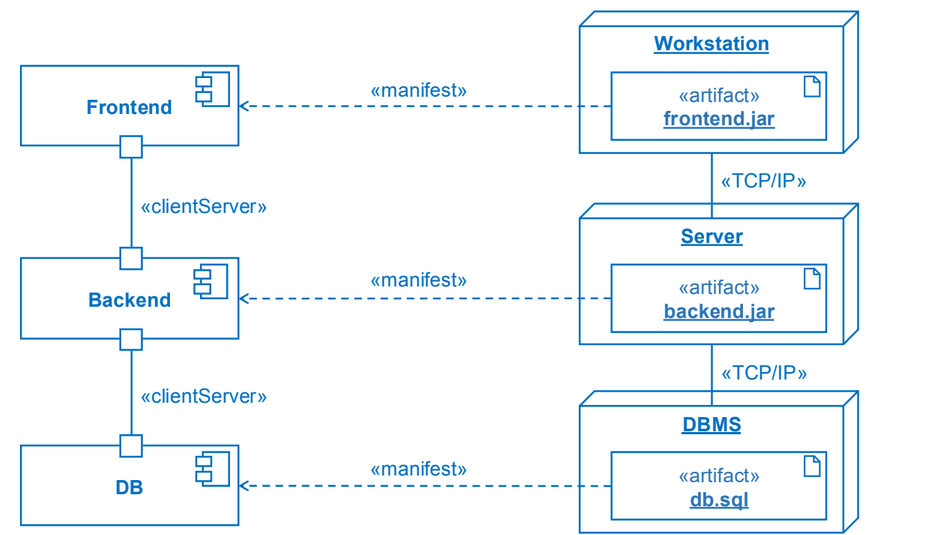
\includegraphics[scale=.4]{ibride}
\end{center}

\subsection{Altri esempi}
\subsubsection{Architettura a livelli}
\begin{wrapfigure}[9]{r}{6cm}
	\vspace{-1cm}
	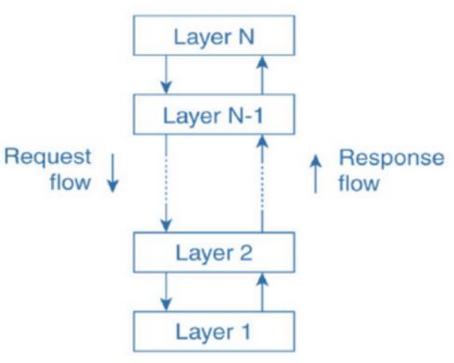
\includegraphics[width=6cm]{livelli}
\end{wrapfigure}
I componenti sono organizzati in livelli (layer) dove uno a livello $i$ può invocarne uno del livello sottostante $i-1$. Le richieste scendono lungo la gerarchia mentre le risposte salgono.

\subsubsection{Architettura multi-livello}
In questa architettura avviene un mapping tra livelli logici (layer) e fisici (tier). Può avere da $1$ ad $N$ livelli, dove all'aumentare di questi si guadagna in \textbf{flessibilità}, \textbf{funzionalità} e possibilità di \textbf{distribuzione} ma si introducono problemi di \textbf{prestazione}. \\
Dal punto di vista fisico, l'architettura può essere:
\begin{itemize}
	\item \textbf{1-tier}: mainframe e terminale
	\item \textbf{2-tier}: macchina client e singolo server
	\item \textbf{3-tier}: ciascun livello su una macchina separate
\end{itemize}
\begin{center}
	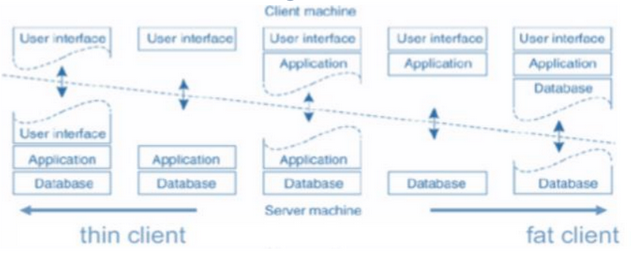
\includegraphics[scale=.4]{multiliv}
\end{center}